\chapter{Ingestion: From PDFs to an Index}
\label{ch:ingestion}

Ingestion turns two PDFs into 3,608 citable passages, each stored with its 768-number embedding. Everything a later citation says --- book, section, printed page --- is decided here. A mistake at this stage makes citations wrong while every later stage appears to work, which is why this code is unusually defensive. It runs as \code{vidyarag download} then \code{vidyarag ingest}, with no API key.

\begin{measured}[a full rebuild from the PDFs]
\code{vidyarag ingest --recreate} into a scratch collection took 1,944\,s (32 minutes) on CPU and reproduced the shipped index exactly.
\begin{center}\small
\begin{tabular}{@{}lrrrr@{}}
\toprule
\textbf{Book} & \textbf{PDF pages} & \textbf{Pages parsed} & \textbf{Chunks} & \textbf{PDF size}\\
\midrule
Biology & 1,480 & 1,273 (86\%) & 1,765 & 279\,MB\\
Anatomy and Physiology & 1,420 & 1,289 (91\%) & 1,843 & 135\,MB\\
\midrule
Total & 2,900 & 2,562 & 3,608 & 415\,MB\\
\bottomrule
\end{tabular}
\end{center}
The resulting index is 34.9\,MB on disk. The repository's own time estimates differ: ``\textasciitilde15 minutes'' in a docstring, and 3,464\,s in \code{docs/EVALUATION.md}. \NotDet{} which conditions produced them.
\end{measured}

\section{The corpus registry}

\code{corpus.py} declares the books once, as frozen \code{BookSpec} records carrying slug, edition, dates, URLs, UUID, ISBN and licence. If \code{ATTRIBUTION.md} ever disagrees with this file, \enquote{this file is what actually ran} \ev{src/vidyarag/ingest/corpus.py}. \textbf{Why exactly these two books?} The licence was checked per title \emph{and per edition}: OpenStax relicensed its second editions as CC~BY-NC-SA, so only these first editions are CC~BY, which ``makes them the complete usable biology corpus rather than a preference among many.'' That was itself a correction. The first corpus commit is titled \enquote{fix(attribution): correct false CC BY claim; switch corpus to CC BY editions.} The licence and source URL are copied onto every stored passage, so attribution ``survives retrieval instead of being bolted on at the UI layer.''

\section{Download}

The downloader promises three properties \ev{src/vidyarag/ingest/download.py}:
\begin{description}[style=sameline,leftmargin=2.6cm,font=\normalfont\bfseries]
  \item[Idempotent.] A PDF already on disk is hashed and counted; the network is not touched.
  \item[Resumable.] An interrupted transfer continues with an HTTP \code{Range} request. The loop handles all three replies: \code{206} appends; \code{200} means the server ignored the range, so it overwrites; \code{416} means a stale partial file, so it is deleted and fetched once from scratch. Each case has a mocked-HTTP test.
  \item[Atomic.] Bytes go to \code{<name>.pdf.part} and are renamed only once complete, so a crash never leaves a truncated file that looks whole.
\end{description}
A manifest records each book's SHA-256, size and page count. Opening the PDF to count pages ``doubles as an integrity check'': a checksum proves the bytes are unchanged, but only opening the file proves it is a PDF rather than an error page. OpenStax publishes no digest, so checksums are \emph{recorded}, not verified, and drift shows only if a person compares a new manifest with an old one \tagI.

\section{Parsing}
\label{sec:parse}

The parser's job is not ``get the text out'' but ``get the text out \emph{and} know where it came from'' \ev{src/vidyarag/ingest/parse.py}.

\paragraph{Structure from the outline, not fonts.} OpenStax PDFs carry a real outline (the bookmarks panel). Guessing headings from font size ``misfires on pull quotes, figure captions, and section headers that happen to wrap, and it fails silently'', so a PDF without an outline raises an error rather than producing citations it cannot justify. \code{load_outline} normalises non-breaking spaces and sorts entries by page. That sort matters: \emph{Biology} ends with a stray ``Blank Page'' entry pointing at page 6, which would otherwise ``swallow the whole book into one bogus range.'' \code{build_structure_map} then assigns every page to the latest outline entry at or before it. The shallowest level is a chapter and resets the section; any deeper entry sets the section.

\paragraph{Exclusions.} Pages under an outline title of preface, index, solutions, answer key, references, appendix, contents or blank page are dropped. ``Solutions'', the roughly 35-page answer key, ``competes for exactly the queries the book should answer and satisfies none of them.'' Exclusion inherits downward but never sideways. The end-of-chapter Glossary is \emph{kept}, because ``key terms are definitions, both of which answer real questions.''

\paragraph{Reading order and cleaning.} Blocks entirely inside the top or bottom 6\% of the page (running heads and footers) are dropped. A column split is detected by sweeping block extents for an uncovered vertical gap that is at least 4\% of the page wide and centred within 18\% of the middle. With two columns, the left column is read fully before the right. The code ranks what each fix prevents: running heads would ``embed as noise on every single chunk'', and naive two-column extraction ``produces text that looks plausible and is actually shredded.'' Hyphenated line breaks are rejoined; end-of-chapter question blocks are cut at their headings; continuation pages with four or more \code{a.}--\code{d.} options are dropped. Removing question sets cut about 8.6\% of chunks.

\begin{finding}[a comment that describes the opposite of its regex --- still open]
The comment says \lstinline~"well-\nknown"~ is \emph{never} rejoined into \code{wellknown}. The pattern \lstinline~([A-Za-z])-\n([a-z])~ does exactly that, because \code{k} is lowercase. What the code actually preserves is a hyphen followed by an \emph{uppercase} letter, and that is what the test checks. The retrieval impact is small, but the comment should not be quoted as behaviour.
\end{finding}

\paragraph{Printed page numbers.} Students look up the number printed on the page, not the PDF index, and these PDFs declare no page labels. \code{printed_page_number} therefore reads the number from the running head, at the start on left-hand pages and at the end on right-hand ones. PDF page 200 of \emph{Biology} is printed page 188, ``and citing 200 would send a reader to the wrong place.'' All 3,608 passages carry a printed page; 61 (1.7\%) have a chapter but no section \tagM.

\section{Chunking}
\label{sec:chunking}

Five rules \ev{src/vidyarag/ingest/chunk.py}. \textbf{(1)} Chunks never cross a section boundary, so their metadata is ``exactly true rather than approximately true.'' \textbf{(2)} They may cross a page break, citing the page where they start. \textbf{(3)} They are built greedily from whole sentences, up to 512 tokens. \textbf{(4)} Consecutive chunks overlap by whole trailing sentences worth at most 64 tokens. \textbf{(5)} Tokens are counted with the embedding model's own tokeniser (Chapter~\ref{ch:concepts}).

\paragraph{Sentence splitting} uses a regex boundary: whitespace after terminal punctuation, optionally followed by a closing quote or bracket, and before a capital letter, an opening quote or bracket, or a digit. The quote classes include typographic quotes, because OpenStax uses them. Twenty abbreviations (\code{e.g}, \code{Fig}, \code{approx}\ldots) are glued back onto the preceding sentence, because Python's look-behind cannot take alternatives of different lengths. \tagI{} A consequence is that a sentence opening in lowercase (``mRNA carries\ldots'', ``pH falls\ldots'') is never split from its predecessor.

\paragraph{Packing.} Each page's text is prefixed with an invisible \code{PAGE:n} marker, so the packer knows which page each sentence starts on. A sentence that alone reaches the budget is emitted on its own. Otherwise sentences accumulate until the next one would overflow. The chunk is then emitted, and the overlap is carried forward (Figure~\ref{fig:packing}).

\begin{figure}[htbp]
\centering
\resizebox{0.95\textwidth}{!}{%
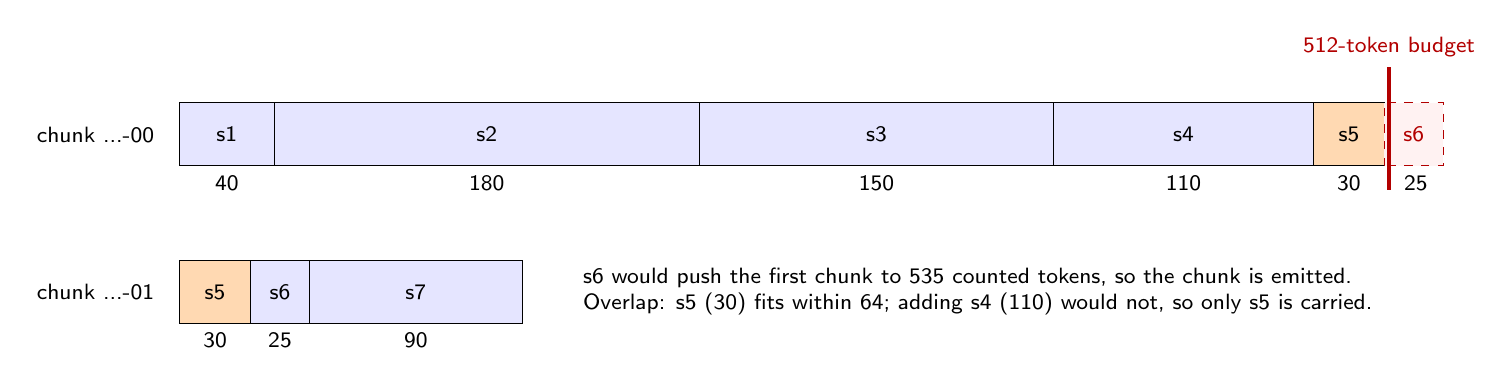
\begin{tikzpicture}[font=\sffamily\footnotesize]
\def\y{1.4}
\draw[fill=blue!10] (0,\y) rectangle (1.2,\y+0.8) node[pos=.5] {s1};
\draw[fill=blue!10] (1.2,\y) rectangle (6.6,\y+0.8) node[pos=.5] {s2};
\draw[fill=blue!10] (6.6,\y) rectangle (11.1,\y+0.8) node[pos=.5] {s3};
\draw[fill=blue!10] (11.1,\y) rectangle (14.4,\y+0.8) node[pos=.5] {s4};
\draw[fill=orange!30] (14.4,\y) rectangle (15.3,\y+0.8) node[pos=.5] {s5};
\draw[dashed, red!70!black, fill=red!5] (15.3,\y) rectangle (16.05,\y+0.8) node[pos=.5] {s6};
\draw[very thick, red!70!black] (15.36,\y-0.3) -- (15.36,\y+1.25) node[above] {512-token budget};
\node[anchor=north] at (0.6,\y) {40}; \node[anchor=north] at (3.9,\y) {180}; \node[anchor=north] at (8.85,\y) {150};
\node[anchor=north] at (12.75,\y) {110}; \node[anchor=north] at (14.85,\y) {30}; \node[anchor=north] at (15.7,\y) {25};
\node[anchor=east] at (-0.2,\y+0.4) {chunk \code{...-00}};
\def\z{-0.6}
\draw[fill=orange!30] (0,\z) rectangle (0.9,\z+0.8) node[pos=.5] {s5};
\draw[fill=blue!10] (0.9,\z) rectangle (1.65,\z+0.8) node[pos=.5] {s6};
\draw[fill=blue!10] (1.65,\z) rectangle (4.35,\z+0.8) node[pos=.5] {s7};
\node[anchor=north] at (0.45,\z) {30}; \node[anchor=north] at (1.275,\z) {25}; \node[anchor=north] at (3.0,\z) {90};
\node[anchor=east] at (-0.2,\z+0.4) {chunk \code{...-01}};
\node[anchor=west, align=left] at (5.0,\z+0.4) {s6 would push the first chunk to 535 counted tokens, so the chunk is emitted.\\Overlap: s5 (30) fits within 64; adding s4 (110) would not, so only s5 is carried.};
\end{tikzpicture}}
\caption{Greedy packing with overlap, with illustrative sentence token counts. Box widths are proportional to tokens.}
\label{fig:packing}
\end{figure}

\begin{measured}[what a token count really measures]
\code{count_tokens("Hello", ...)} returns 3 (\code{[CLS] hello [SEP]}), and a 1,000-word string returns exactly 512, because the tokeniser truncates. \tagI{} So every sentence's cost includes two special tokens that the joined chunk contains only once, and chunks are packed as if $2(n-1)$ tokens longer than they are. That is consistent with the maximum chunk being 487 tokens rather than 512.
\end{measured}

\begin{center}\small
\begin{tabular}{@{}lr@{\qquad}lr@{}}
\toprule
Mean / median tokens & 428 / 455 & Chunks under 120 tokens & 70\\
5th / 95th percentile & 206 / 475 & Spanning more than one page & 1,990 (55\%)\\
Minimum / maximum & 44 / 487 & From Glossary sections & 594 (16.5\%)\\
\bottomrule
\end{tabular}
\end{center}

Chunk ids are \texttt{\{slug\}-p\{start:04d\}-\{seq:02d\}}, such as \code{biology-p0388-01}. They cannot collide, because a page belongs to exactly one section and the sequence counter runs within a section. A stored citation reads \code{Biology, 14.4. DNA Replication in Prokaryotes*, p.376}; the asterisk is part of the outline's title.

\begin{measured}[where chunking shows: ``what is tissue?'']
The top hit was \emph{Anatomy and Physiology}, 4.1 Types of Tissues, p.136. It is the right section, but the passage begins mid-sentence and contains no one-line definition. The crisp definitions sit in Glossary passages that did not reach the top five. \code{docs/EVALUATION.md} lists this under ``What did not work'', and the README names short definitional questions as a known weakness that the gold set under-samples.
\end{measured}

\section{Embedding and storage}
\label{sec:store}

The embedder is cached per process, because building it costs far more than using it; the first call downloads about 210\,MB of ONNX weights. Ingestion embeds and upserts in batches of 64. The collection design has four properties \ev{src/vidyarag/store/collection.py}:
\begin{description}[style=nextline]
  \item[Deterministic ids.] \code{uuid5(POINT_NAMESPACE, chunk_id)} gives the same id on every machine, so a rewrite overwrites. Random ids ``would silently double the corpus and quietly wreck every retrieval metric that follows.''
  \item[A named vector, \code{dense}.] This leaves room for a sparse vector beside it. Hybrid search was never built, but renaming later would orphan every point.
  \item[Dimension mismatches fail early,] with a message telling you to re-ingest with \code{--recreate}, rather than failing ``deep inside an upsert''.
  \item[A 13-field payload] per point: id, book slug and title, chapter, section, page range, printed page, citation, text, token count, licence and source URL.
\end{description}

\paragraph{The orchestrator} \ev{src/vidyarag/ingest/pipeline.py} scrolls the collection for existing chunk ids, in pages of 1,000, and skips them. It reads ids rather than trusting a count, because ``only the ids say which chunks still need work.'' Parsing and chunking always rerun; only embedding is skipped. It finishes by writing an \code{IngestReport} to \code{data/ingest_run.<collection>.json}. Before the fixes this was one fixed \code{data/ingest_run.json}, which any other build silently overwrote. That happened during this analysis, when a scratch rebuild replaced the working index's provenance.

\paragraph{Still open:} \code{store/client.py} still explains its 20,000-point threshold by a corpus ``expected to land near 6k chunks''. It is 3,608.
